\section{Du booléen au circuit}

\begin{frame}{Portes élémentaires}

    Chaque opération booléenne correspond à une \textbf{porte logique} physique, \textit{pour peu qu'elle ait été conçue par le fondeur} (au niveau transistor).

    \vspace{0.5cm}

    \centering
    \begin{tabular}{|c|c|c|}
        \hline
        \textbf{Opération} & \textbf{Symbole} & \textbf{Porte logique} \\
        \hline
        Négation & \(\bar{x}\) & NOT \\
        Conjonction & \(x \cdot y\) & AND2 \\
        Disjonction & \(x + y\) & OR2 \\
        Disjonction & \(x + y + z\) & OR3 \\

        \hline
    \end{tabular}

    \vspace{0.6cm}

    \begin{block}{Portes universelles}
        Les portes \textbf{NAND} et \textbf{NOR} sont dites \textit{universelles} : toute fonction booléenne peut être réalisée à partir de l'une d'elles uniquement.
    \end{block}

    \vspace{0.3cm}
    \centering
    \textit{L'algèbre de Boole est le langage mathématique de l'électronique numérique.}

\end{frame}



\begin{frame}{Portes logiques : symboles usuels}
  \begin{center}
    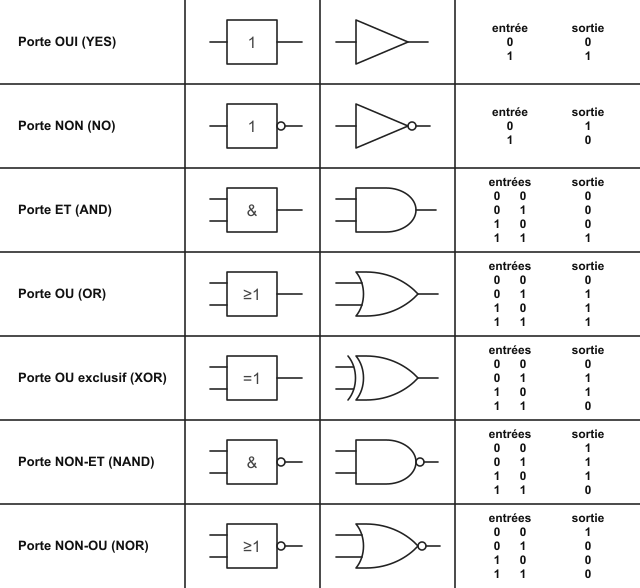
\includegraphics[scale=0.45]{./images/portes_logiques.png}
  \end{center}
\end{frame}


\begin{frame}{Portes Logiques : du Booléen au Modèle Physique}

    %\vspace{0.3cm}

    \begin{columns}[T]
        \begin{column}{0.52\textwidth}
          \begin{block}{Définition  (tentative) — Porte logique }
            Une \textbf{porte logique} à \(k\) entrées est un triplet :
            \[
            g = (f_g, \tau_g, A_g)
            \]
            où :
            \begin{itemize}
              \item \(f_g : \mathbb{B}^k \to \mathbb{B}\) est la \textbf{fonction réalisée} ;
              \item \(\tau_g \geq 0\) est le \textbf{délai de propagation} (temps) ;
              \item \(A_g \geq 0\) est la \textbf{surface} occupée (espace).
            \end{itemize}
          \end{block}
            \textbf{Modèle d'un circuit combinatoire}\\[0.2cm]
            Un circuit est un \textbf{graphe orienté acyclique} (DAG) :
            \[
                G = (V, E)
            \]
            \begin{itemize}
                \item \(V\) : portes \(\cup\) entrées \(\cup\) sorties ;
                \item \(E \subseteq V \times V\) : fils (connexions).
            \end{itemize}

            \vspace{0.2cm}
            La fonction globale \(F : \mathbb{B}^n \to \mathbb{B}^m\) est obtenue par \textbf{composition} le long du DAG.
        \end{column}
        \begin{column}{0.45\textwidth}
            \centering
            \renewcommand{\arraystretch}{1.2}
            \begin{tabular}{|c|c|c|c|}
                \hline
                \textbf{Porte} & \textbf{Fonction} & \(A\) (µm²) & \(\tau\) (ns) \\
                \hline
                INV   & \(\bar{a}\)            & 1 & 0.05 \\
                NAND2 & \(\overline{ab}\)      & 2 & 0.08 \\
                NOR2  & \(\overline{a+b}\)     & 2 & 0.09 \\
                AND2  & \(ab\)                 & 3 & 0.13 \\
                OR2   & \(a+b\)                & 3 & 0.14 \\
                XOR2  & \(a \oplus b\)         & 6 & 0.22 \\
                \hline
            \end{tabular}
            \vspace{0.2cm}

            {\footnotesize Chiffres indicatifs (nœud technologique générique).}

            \begin{alertblock}{Circuit Combinatoire}
              Pas de cycle = pas de rebouclage.
            \end{alertblock}
        \end{column}
    \end{columns}

    \vspace{0.2cm}

    \begin{alertblock}{Rupture conceptuelle}
        \centering
        On passe d'une fonction \textbf{intemporelle} \(f : \mathbb{B}^n \to \mathbb{B}\) à un objet \textbf{coûteux} : chaque porte a un prix en temps et en surface.
    \end{alertblock}

\end{frame}
%
% % --- Frame : Netlist et hiérarchie ---
% \begin{frame}{Netlist et Hiérarchie : la Structure Formelle d'un Circuit}
%
%     \begin{block}{Définition — Netlist}
%         Une \textbf{netlist} est un triplet :
%         \[
%             \mathcal{N} = (V, N, \pi)
%         \]
%         où :
%         \begin{itemize}
%             \item \(V\) est un ensemble d'\textbf{instances} de cellules ;
%             \item \(N\) est un ensemble de \textbf{nets} (fils) ;
%             \item \(\pi : V \to N^*\) associe à chaque instance ses ports connectés.
%         \end{itemize}
%     \end{block}
%
%     \vspace{0.3cm}
%
%     \begin{columns}[T]
%         \begin{column}{0.5\textwidth}
%             \begin{alertblock}{Définition — Module hiérarchique}
%                 Un \textbf{module} est un couple :
%                 \[
%                     M = (\text{ports},\, \text{implémentation})
%                 \]
%                 où l'implémentation est elle-même une netlist (récursion).
%             \end{alertblock}
%
%             \vspace{0.2cm}
%
%             \textbf{Encapsulation :} l'interface (ports) cache l'implémentation.\\
%             \textit{Principe de boîte noire :}\\
%             \[
%                 M : \mathbb{B}^{p} \to \mathbb{B}^{q}
%             \]
%         \end{column}
%         \begin{column}{0.48\textwidth}
%             \textbf{Exemple — Additionneur 8 bits :}
%
%             \vspace{0.3cm}
%
%             \centering
%             \begin{tikzpicture}[
%                 scale=0.7,
%                 every node/.style={draw, rounded corners, minimum height=0.6cm, font=\footnotesize}
%             ]
%                 \node (top) at (0, 2.5) {Top};
%                 \node (add8) at (0, 1.5) {Adder8};
%                 \node (a4a) at (-1.6, 0.4) {Adder4};
%                 \node (a4b) at (1.6, 0.4) {Adder4};
%                 \node (fa1) at (-2.4, -0.7) {FA};
%                 \node (fa2) at (-1.0, -0.7) {FA};
%                 \node (fa3) at (0.8, -0.7) {FA};
%                 \node (fa4) at (2.2, -0.7) {FA};
%
%                 \draw (top) -- (add8);
%                 \draw (add8) -- (a4a);
%                 \draw (add8) -- (a4b);
%                 \draw (a4a) -- (fa1);
%                 \draw (a4a) -- (fa2);
%                 \draw (a4b) -- (fa3);
%                 \draw (a4b) -- (fa4);
%             \end{tikzpicture}
%         \end{column}
%     \end{columns}
%
%     \vspace{0.2cm}
%
%     \begin{exampleblock}{Instanciation et réutilisation}
%         \centering
%         \(\text{Adder8} = \text{Adder4} \circ \text{Adder4}\) — la composition de modules préserve la fonction et divise la complexité.
%     \end{exampleblock}
%
% \end{frame}
%
% % --- Frame : Chemin critique et fréquence ---
% \begin{frame}{Chemin Critique et Fréquence de Fonctionnement}
%
%     \begin{block}{Modèle temporel}
%         À chaque porte \(v \in V\), on associe un délai \(\tau_v \geq 0\).
%
%         Le \textbf{délai d'un chemin} \(P = (v_0, v_1, \dots, v_k)\) est :
%         \[
%             T(P) \;=\; \sum_{i=0}^{k} \tau_{v_i}
%         \]
%     \end{block}
%
%     \vspace{0.3cm}
%
%     \begin{alertblock}{Définition — Chemin critique}
%         Le \textbf{chemin critique} est le chemin de délai maximal entre une entrée et une sortie :
%         \[
%             T_{\text{crit}} \;=\; \max_{P \in \mathcal{P}} \; T(P)
%         \]
%         où \(\mathcal{P}\) désigne l'ensemble des chemins entrée \(\to\) sortie.
%     \end{alertblock}
%
%     \vspace{0.3cm}
%
%     \begin{columns}[T]
%         \begin{column}{0.52\textwidth}
%             \textbf{Fréquence maximale} (modèle combinatoire pur) :
%             \[
%                 f_{\max} \;=\; \frac{1}{T_{\text{crit}}}
%             \]
%
%             \vspace{0.3cm}
%
%             \textbf{Slack} d'un chemin \(P\) :
%             \[
%                 s(P) \;=\; T_{\text{requis}} - T(P)
%             \]
%             \begin{itemize}
%                 \item \(s(P) = 0\) : chemin critique ;
%                 \item \(s(P) > 0\) : marge disponible.
%             \end{itemize}
%         \end{column}
%         \begin{column}{0.45\textwidth}
%             \begin{exampleblock}{Interprétation algorithmique}
%                 Le calcul de \(T_{\text{crit}}\) se fait en \(O(|V| + |E|)\) par :
%                 \begin{enumerate}
%                     \item tri topologique du DAG ;
%                     \item propagation des délais en avant (plus long chemin).
%                 \end{enumerate}
%
%                 \vspace{0.2cm}
%                 C'est un \textbf{plus long chemin dans un DAG} — problème classique de théorie des graphes.
%             \end{exampleblock}
%         \end{column}
%     \end{columns}
%
%     \vspace{0.2cm}
%
%     \begin{block}{Problème d'optimisation temporelle}
%         \centering
%         Maximiser le \textbf{slack minimum} sous contrainte de préservation de la fonction :
%         \[
%             \max_{G'} \; \min_{P} \; s(P) \quad \text{s.c.} \quad F_{G'} = F_{G}, \quad A_{G'} \leq A_{\max}
%         \]
%     \end{block}
%
% \end{frame}

\begin{frame}
\frametitle{Mapping technologique : de l'équation booléenne à la structure}

\vspace{0.2cm}

\begin{center}
\begin{tikzpicture}[
    node distance=1.6cm,
    box/.style={draw=black!70, rounded corners=2pt,
                minimum width=3.6cm, minimum height=1.1cm,
                align=center, font=\small},
    arr/.style={-{Latex[length=2.5mm]}, thick, black!70}
]

\node[box] (eq) {\textbf{Équations booléennes}\\[2pt]
                  $f = \overline{a}\,b + c\,(\overline{a} + d)$};

\node[box, right=of eq] (lib) {\textbf{Bibliothèque fondeur}\\[2pt]
                  \texttt{AND2, OR2, INV, NAND2, \dots}};

\node[box, right=of lib] (net) {\textbf{Structure effective}\\[2pt]
                  netlist / layout};

\draw[arr] (eq) -- node[above, font=\scriptsize]{simplification}
                 node[below, font=\scriptsize]{Mapping} (lib);
\draw[arr] (lib) -- node[above, font=\scriptsize]{connexion} (net);

\end{tikzpicture}
\end{center}

\vspace{0.35cm}

\begin{columns}[T]
\begin{column}{0.48\textwidth}
\textbf{Entrées du mapping}
\begin{itemize}\setlength\itemsep{2pt}
    \item Équations booléennes optimisées
    \item Bibliothèque de cellules (\emph{std cells})
    \item Reformulation selon disponibilité des cellules.
    \item Contraintes : aire, délai, fanout
\end{itemize}
\end{column}

\begin{column}{0.48\textwidth}
\textbf{Sortie effective}
\begin{itemize}\setlength\itemsep{2pt}
    \item Réseau de cellules interconnectées
    \item Respect des \emph{design rules}
    \item Prêt pour placement/routage
\end{itemize}
\end{column}
\end{columns}

\vfill
\begin{center}
\footnotesize\itshape
Le mapping traduit une expression logique en une réalisation physique contrainte par la bibliothèque du fondeur.
\end{center}

\end{frame}

% --- Frame : Porte, ports, instance ---
\begin{frame}{Circuit : tentative de définition formelle}

    \begin{block}{Définition — Port}
        Un \textbf{port} est un objet typé :
        \[
            p = (\text{nom},\, \text{direction},\, \text{largeur})
        \]
        avec \(\text{direction} \in \{in, out\}\) et \(\text{largeur} \in \mathbb{N}^*\).
    \end{block}

    \vspace{0.2cm}

    \begin{block}{Définition — Circuit (combinatoire)}
        Un \textbf{circuit} combinatoire est la donnée : $g = (\text{name},\, P_g,\, f_g,\, \tau_g,\, A_g)$
        % \[
        %     g = (\text{name},\, P_g,\, f_g,\, \tau_g,\, A_g)
        % \]
        où :
        \begin{itemize}
            \item \(P_g = P_g^{in} \uplus P_g^{out}\) : ensemble de ports, partitionné en entrées / sorties ;
            \item \(f_g : \mathbb{B}^{|P_g^{in}|} \to \mathbb{B}^{|P_g^{out}|}\) : fonction booléenne générale;
            \item \(\tau_g \in \mathbb{R}_{\geq 0}\) : délai caractéristique ;
            \item \(A_g \in \mathbb{R}_{\geq 0}\) : surface.
        \end{itemize}
    \end{block}

    % \vspace{0.1cm}
    %
    % \begin{columns}[T]
    %     \begin{column}{0.55\textwidth}
    %         \begin{alertblock}{Exemple — NAND2}
    %             \(P_g^{in} = \{a, b\}\), \; \(P_g^{out} = \{y\}\)\\[0.2cm]
    %             \(f_g(a,b) = \overline{a \cdot b}\), \quad \(\tau_g = 0.08\) ns, \quad \(A_g = 2\) µm²
    %         \end{alertblock}
    %     \end{column}
    %     \begin{column}{0.42\textwidth}
    %         \centering
    %         \begin{tabular}{|c|c|c|c|}
    %             \hline
    %             \textbf{Porte} & \(\tau\) (ns) & \(A\) (µm²) & Ports \\
    %             \hline
    %             INV   & 0.05 & 1 & \(\{a\} / \{y\}\) \\
    %             NAND2 & 0.08 & 2 & \(\{a,b\} / \{y\}\) \\
    %             NOR2  & 0.09 & 2 & \(\{a,b\} / \{y\}\) \\
    %             XOR2  & 0.22 & 6 & \(\{a,b\} / \{y\}\) \\
    %             \hline
    %         \end{tabular}
    %     \end{column}
    % \end{columns}

\end{frame}

% --- Frame : Netlist comme interconnexion de ports ---
\begin{frame}{Netlist : Interconnexion de Ports}

    \begin{block}{Définition — Instance de circuit}
        Une \textbf{instance} d'un circuit \(c\) \textbf{modèle} est un triplet :
        \[
            i = (c,\, \text{id},\, \sigma_i)
        \]
        où \(\sigma_i : P_c \to N\) associe chaque port de \(c\) à un \textbf{net} (\textit{fil}, \textit{wire}).

        Les ports de l'instance sont notés : \(\text{Ports}(i) = \{(i,p) \mid p \in P_c\}\).
    \end{block}

    \vspace{0.1cm}

    \begin{alertblock}{Définition — Netlist}
        Une \textbf{netlist} est un quadruplet $\mathcal{N} = (I,\, N,\, \Sigma,\, \text{io})$
        % \[
        %     \mathcal{N} = (I,\, N,\, \Sigma,\, \text{io})
        % \]
        où :
        \begin{itemize}
            \item \(I\) : ensemble d'instances ;
            \item \(N\) : ensemble de nets ;
            \item \(\Sigma = \{\sigma_i\}_{i \in I}\) : connexions port \(\to\) net ;
            \item \(\text{io}\) : ports externes de l'interface.
        \end{itemize}
    \end{alertblock}

\end{frame}



\begin{frame}{Exemple : netlist élémentaire}
  \begin{center}
    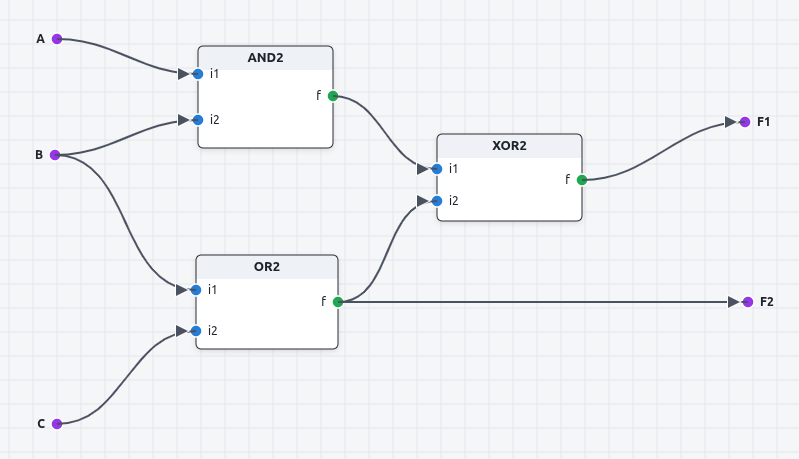
\includegraphics[scale=0.3]{./images/netlist_1.png}
  \end{center}
  Notes :
  \begin{itemize}
    \item partage de ressources (ici \texttt{OR2}) entre 2 fonctions $F1$ et $F2$
  \end{itemize}
\end{frame}

\begin{frame}{Exemple : introduction de hiérarchie}
  \begin{center}
    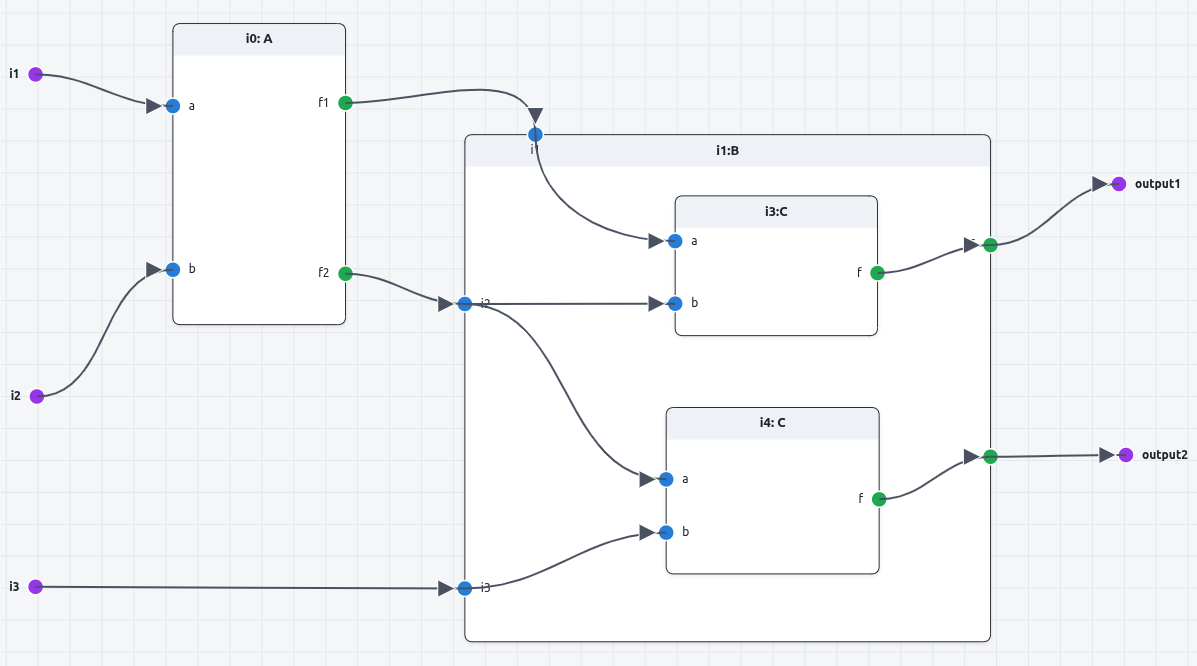
\includegraphics[scale=0.25]{./images/netlist_2.png}
  \end{center}
  Notes :
  \begin{itemize}
    \item \texttt{i3} et \texttt{i4} sont des \textit{instance} d'un modèle composant (modèle) \texttt{C}.
  \end{itemize}
\end{frame}

\begin{frame}{Compléments : signaux directionnels et encapsulation}
  \begin{columns}[T]
    \begin{column}{0.55\textwidth}
      \textbf{Signaux \textit{pilotés} :}
      \begin{enumerate}
        \item \textbf{Connexion} : tout net est piloté par un port (\textit{driver}).
        \item \textbf{Fanout} : un port pilote un ou plusieurs nets.
        \item \textbf{Risques} : un port piloté par plusieurs drivers conduit à un court-circuit et la destruction du circuit...
        %\item \textbf{Largeur} : tous les ports d'un même net ont même largeur.
      \end{enumerate}
    \end{column}
    \begin{column}{0.42\textwidth}
      \textbf{Mécanisme d'Encapsulation:}
      \begin{enumerate}
        \item Une fois le circuit constitué, on peut le refermer.
        \item Sa fonction reste la même, quelle que soient les interactions externes.
        \item (Ce n'est pas vrai pour un circuit analogique. Pas de "fonction")
      \end{enumerate}

    \end{column}
  \end{columns}
  \begin{exampleblock}{Approche constructive}
    Un circuit, construit à partir d'instances d'autres circuits, peut lui-même être instancié par la suite, etc.
    \begin{itemize}
      \item L'exemplaire du modèle devient un modèle, etc.
      \item Une fonction logique peut devenir un composant réutilisable, puis être composée avec d’autres
fonctions, sans réintroduire leur physique interne.
    \end{itemize}
  \end{exampleblock}
\end{frame}


\begin{frame}{De la contrainte physique au contrat comportemental}

  \begin{columns}[T]

  %------------------------------------------------
  \column{0.47\textwidth}

  \begin{block}{Analogique : une relation}
  Un composant impose une \alert{contrainte} entre les
  grandeurs de son environnement :
  \[
          F(V,I)=0
  \]

  %\vspace{0.1cm}

  Tensions et courants restent
  \emph{couplés} : le comportement du composant dépend
  de ce qui lui est connecté.

  %\medskip

  \centering
  \[
  \boxed{\text{``lot de contraintes''}}
  \]
  \centering
  \[
  \boxed{\text{``Approche acausale''}}
  \]

  \end{block}

  %------------------------------------------------
  \column{0.47\textwidth}

  \begin{block}{Numérique : une fonction}
  L'encapsulation logique transforme une entrée en une
  \alert{sortie} :

  \[
          Y=f(A,B,\ldots)
  \]

  %\vspace{0.1cm}

  Le détail physique est masqué derrière les niveaux
  logiques et leurs marges.

  \medskip

  \centering
  \[
  \boxed{\text{``lot de garanties''}}
  \]
  \[
  \boxed{\text{``Approche causale''}}
  \]
  \end{block}

  \end{columns}

  %\vspace{0.1cm}

  % \begin{alertblock}{La puissance constructive du numérique}
  % Une fonction logique peut devenir \alert{un composant
  % réutilisable}, puis être composée avec d'autres fonctions,
  % sans réintroduire leur physique interne.
  % \end{alertblock}
\end{frame}

% --- Frame : Chemin critique via les ports ---
\begin{frame}{Chemin Critique : Définition via les Ports}

    \begin{block}{Définition — Chemin}
        Un \textbf{chemin} dans une netlist est une séquence alternée de ports :
        \[
            P = (i_0, p_0) \to (i_1, p_1) \to \dots \to (i_k, p_k)
        \]
        telle que :
        \begin{itemize}
            \item \((i_j, p_j)\) est un port de \textbf{sortie} de \(g_{i_j}\) ;
            \item \((i_{j+1}, p_{j+1})\) est un port d'\textbf{entrée} de \(g_{i_{j+1}}\) ;
            \item \(\sigma_{i_j}(p_j) = \sigma_{i_{j+1}}(p_{j+1})\) (même net).
        \end{itemize}
    \end{block}

    \vspace{0.2cm}

    \begin{block}{Délai d'un chemin}
        \[
            T(P) \;=\; \sum_{j=0}^{k} \tau_{g_{i_j}}
        \]
    \end{block}
\end{frame}

\begin{frame}{Chemin critique}
  \begin{columns}
    \begin{column}{0.6\textwidth}
      \begin{alertblock}{Chemin critique et fréquence}
        \[
        T_{\text{crit}} \;=\; \max_{P \in \mathcal{P}} T(P), \qquad f_{\max} \;=\; \frac{1}{T_{\text{crit}}}
        \]
        où \(\mathcal{P}\) parcourt les chemins allant d'un port externe d'entrée à un port externe de sortie.
      \end{alertblock}

      \vspace{0.1cm}

      \begin{exampleblock}{Calcul algorithmique}
        \centering
        Le calcul se fait en \(O(|I| + |\Sigma|)\) par tri topologique du DAG des instances : c'est un \textbf{plus long chemin} dans un DAG.
      \end{exampleblock}
    \end{column}

    \begin{column}{0.4\textwidth}
      \begin{center}
        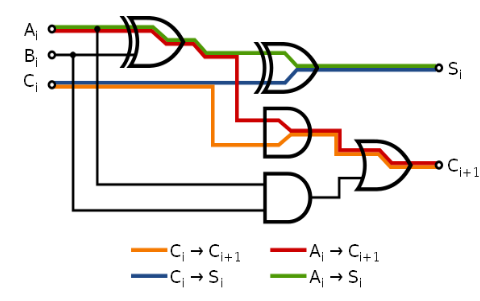
\includegraphics[scale=0.3]{./images/netlist_3.png}
      \end{center}
    \end{column}
  \end{columns}

\end{frame}



\begin{frame}{Circuits reconfigurables : FPGA}
  \begin{columns}[T]
    \begin{column}{0.5\textwidth}
      \begin{itemize}
        \item Coût élevé d'un circuit \textbf{ASIC} \textit{custom}...
        \item \textbf{FPGA} (1985) : circuit \textit{reconfigurable} à volonté.
        \begin{itemize}
          \item Approche \textit{Software-like} \footnote{voir TD \texttt{LUT2} où la notion de \textit{bitstream} sera expliquée.}
          \item Parallélisme équationnel booléen \textit{massif}.
        \end{itemize}
        \item Excellents pour :
        \begin{itemize}
          \item Prototypage, expérimentation.
          \item Faible volume de production.
          \item Fréquences de fonctionnement modérées.
          \item Existent aussi sous forme d'IP.
        \end{itemize}
        \item Fournisseurs :
        \begin{itemize}
          \item Xilinx (AMD), Altera (Intel)
          \item Lattice, Microchip (Microsemi)
          \item \textit{noeuds} technologiques avancés
          \item Equivalent de millions de portes logiques.
        \end{itemize}
      \end{itemize}
    \end{column}
    \begin{column}{0.5\textwidth}
      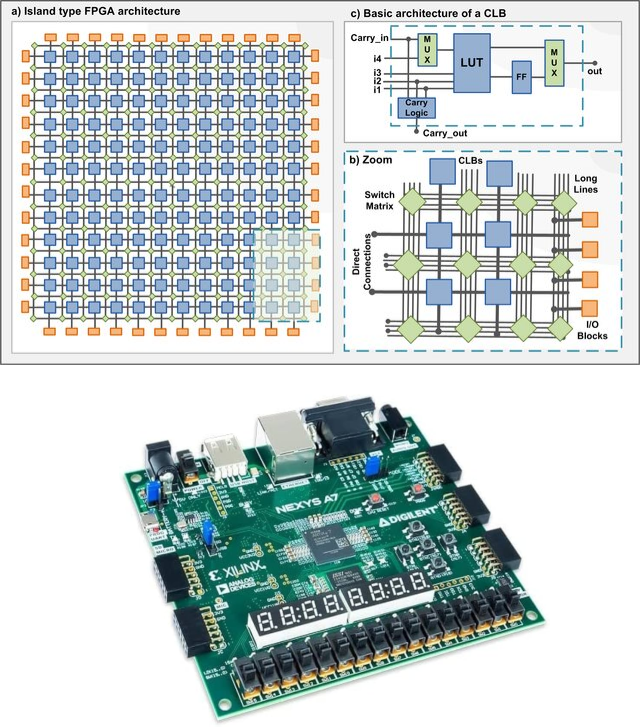
\includegraphics[scale=0.34]{./images/fpga_1.png}
    \end{column}
  \end{columns}
\end{frame}

\begin{frame}{FPGA : loin des circuits discrets !}
  \begin{center}
    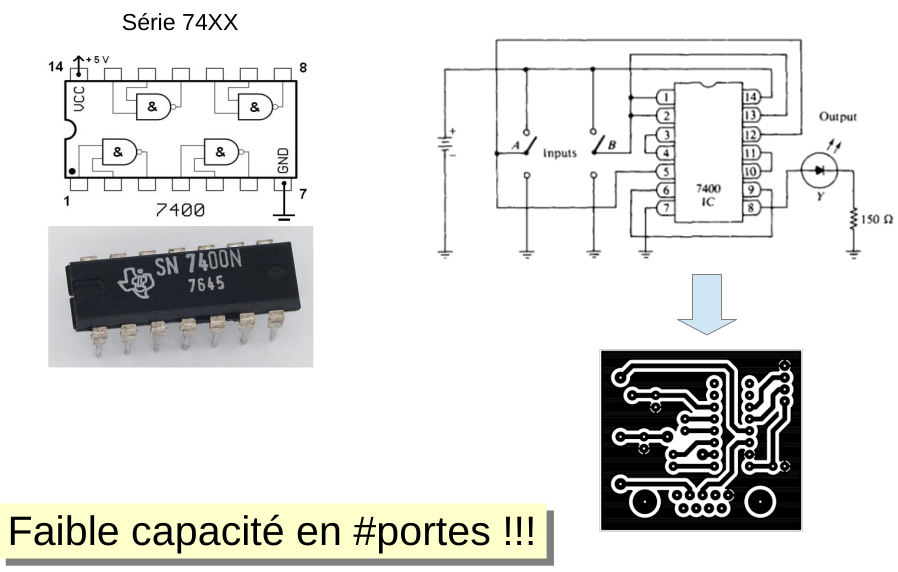
\includegraphics[scale=0.3]{./images/mapping.png}
  \end{center}
\end{frame}
